\documentclass{article}
\usepackage{tikz}
\usepackage{tikz-3dplot}

\begin{document}

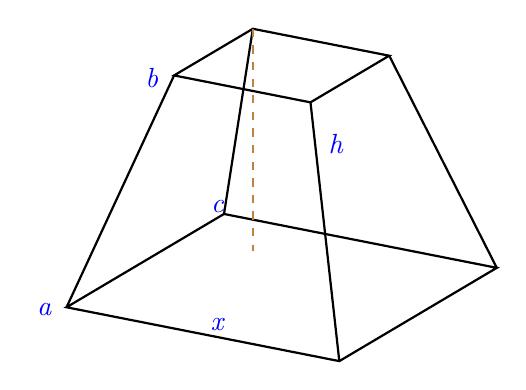
\begin{tikzpicture}

% Define perspective transformation
\tdplotsetmaincoords{70}{120}
\begin{scope}[tdplot_main_coords]

% Define the bottom base coordinates
\coordinate (A) at (-2,-2,0);
\coordinate (B) at (2,-2,0);
\coordinate (C) at (2,2,0);
\coordinate (D) at (-2,2,0);

% Define the top base coordinates
\coordinate (E) at (-1,-1,3);
\coordinate (F) at (1,-1,3);
\coordinate (G) at (1,1,3);
\coordinate (H) at (-1,1,3);

\coordinate (El) at (-1,-1,0);
\coordinate (Fl) at (1,-1,0);
\coordinate (Gl) at (1,1,0);
\coordinate (Hl) at (-1,1,0);

% Draw the solid edges
\draw[thick] (A) -- (B) -- (C) -- (D) -- cycle; % Bottom base
\draw[thick] (E) -- (F) -- (G) -- (H) -- cycle; % Top base
\draw[thick] (A) -- (E);
\draw[thick] (B) -- (F);
\draw[thick] (C) -- (G);
\draw[thick] (D) -- (H);

% Draw the correct dashed lines (hidden edges)
\draw[dashed, brown, thick] (E) -- (El); % Vertical hidden edge

% Add labels in blue italics
\node[blue] at (-2.2,-2.2,0) {\textit{c}};
\node[blue] at (2.2,-2.2,0) {\textit{a}};
\node[blue] at (1.2,-1.2,3) {\textit{b}};
\node[blue] at (-1.4,0,1.5) {\textit{h}};
\node[blue] at (1.6,0,0) {\textit{x}};

\end{scope}
\end{tikzpicture}

\end{document}
